% !TEX root = ../../../main.tex
% 来源：中学数学实验教材·第三册（高中数学）
% 章节：函数及其图象 / 函数及其图象
% 原始文件：4.tex，行 914-923
% 类型：tikz
% ---
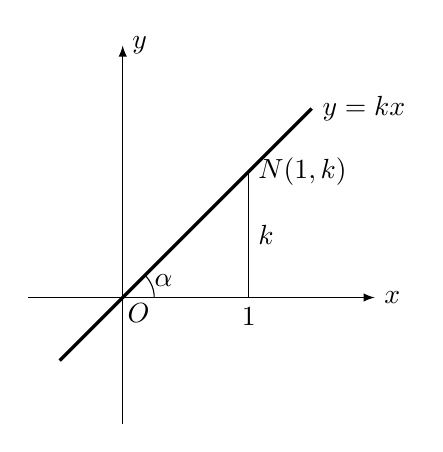
\begin{tikzpicture}[>=latex, scale=.8]
    \draw[->](-1.5,0)--(4,0)node[right]{$x$};
    \draw[->] (0,-2)--(0,4)node[right]{$y$};
\draw[very thick] (-1,-1)--(3,3)node[right]{$y=kx$};
\draw (2,0)node[below]{1}--(2,.1);
\draw (2,0)--node[right]{$k$}(2,2)node[right]{$N(1,k)$};
\node at (.25,-.25){$O$};
\draw (.5,0) arc (0:45:.5); 
\node at (22.5:.7){$\alpha$};
\end{tikzpicture}
